The purpose of this chapter is to explain the technical details of the MicroBooNE detector. An understanding of how a liquid argon time projection chamber like MicroBooNE works is crucial for understanding the results of analyses described in later chapters. Using this specific detector technology gives rise to certain backgrounds in measurements which are relevant to MicroBooNE that may not be relevant for other experiments using different detection techniques, like MiniBooNE. Additionally, understanding how the detector works sheds light on what detector-specific uncertainties are present in MicroBooNE analyses.

\section{Introduction}
The MicroBooNE (the Micro Booster Neutrino Experiment) detector \cite{UBDetectorPaper} is a $\sim$60 ton fiducial mass (170 ton total mass) liquid argon time projection chamber (LArTPC) contained within a cylindrical cryostat, located on-axis of the Booster Neutrino Beam-line (BNB) 470 meters downstream from the neutrino production target at the Fermi National Accelerator Laboratory (FNAL) in Batavia, Illinois. A schematic of how a LArTPC works is shown in Figure \ref{LArTPC_concept_fig}. A LArTPC involves a detector medium in an external electric field. Particles traversing the medium both create scintillation light, which are observed by photomultiplier tubes (PMTs, not shown in Figure \ref{LArTPC_concept_fig}) and leave trails of ionization electrons. These ionization electrons are drifted by the electric field past a number of closely spaced wire planes at different pitch angles. The signals generated in each plane as the electrons either pass close to wires or are collected on wires are what are used to create a two-dimensional image of the event. Combining information from multiple planes along with that from the PMTs allows for the creation of three-dimensional reconstructions of the event. Additionally, the relative size of the signals on the wire planes provide calorimetric information, which is used for particle identification capabilities.\\

The main components of the MicroBooNE TPC (the TPC, the light collection system, and the readout and triggering system) are described in the following sections.

\begin{figure}[ht!]
\centering
	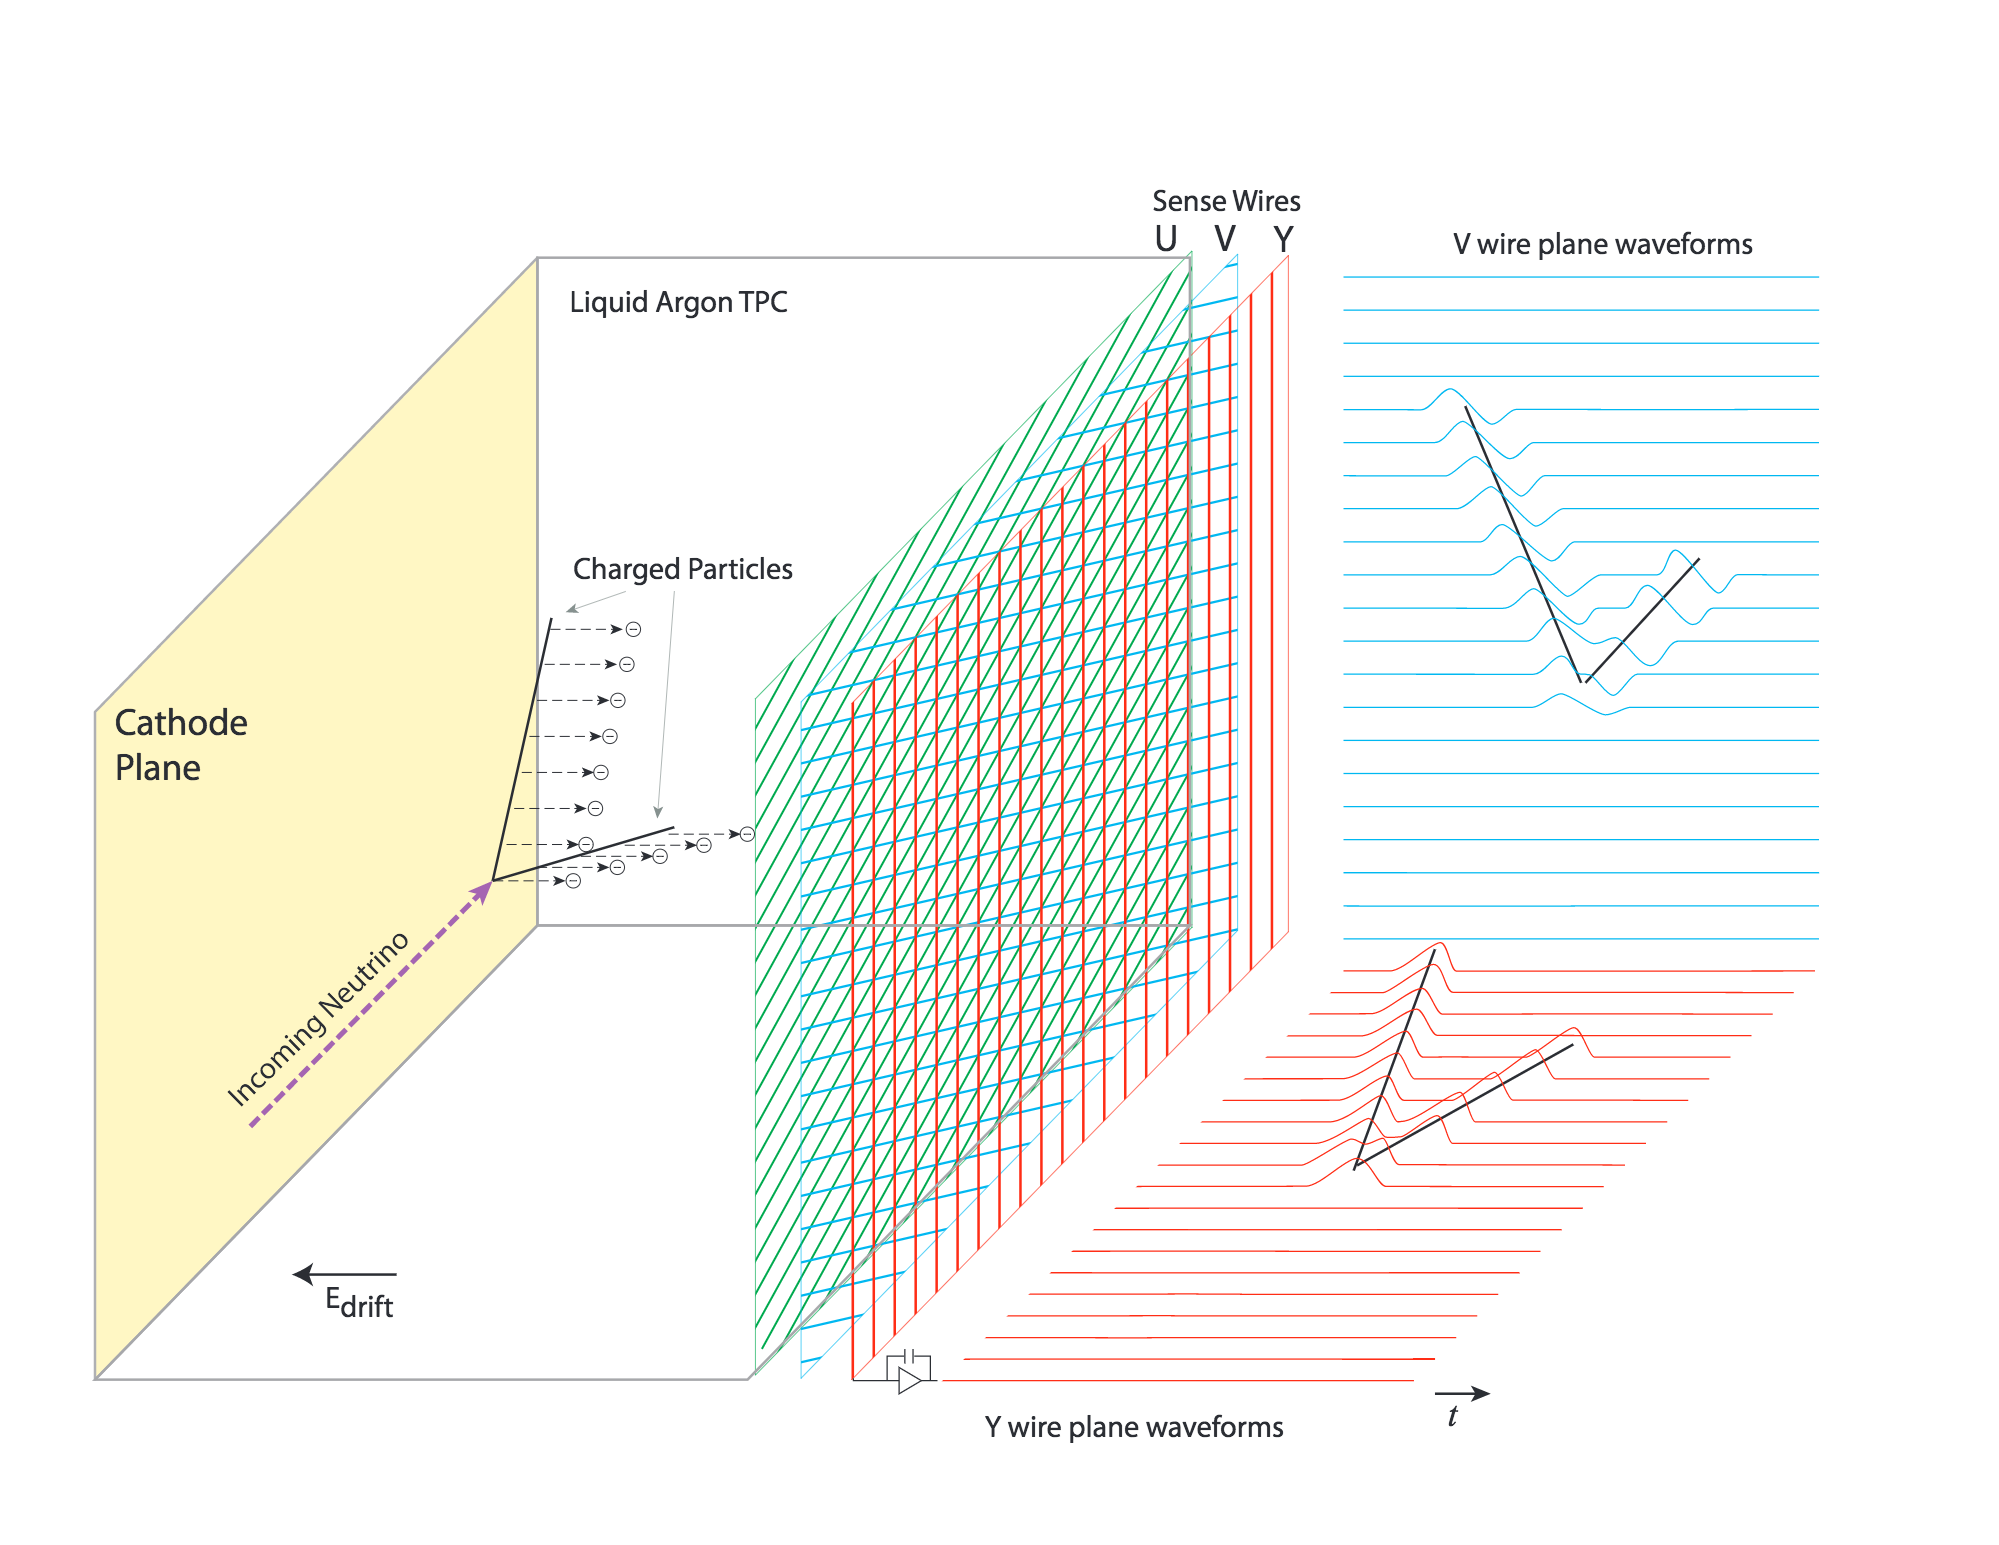
\includegraphics[width=0.9\textwidth]{Figures/LArTPC_concept.png} \\
\caption{\textit{A cartoon schematic of how a LArTPC works. Ionization electrons from particles traversing the detector medium are drifted by an electric field, $E_{\text{drift}}$ past multiple planes of sense wires. The signals on those wires create several two-dimensional images of the event, which are combined to create a three-dimensional reconstruction of the event. Note that in a LArTPC, PMTs are used to collect scintillation light, but are not drawn in this diagram.}}\label{LArTPC_concept_fig}
\end{figure}


\section{Time Projection Chamber}
The time projection chamber (TPC) used in the MicroBooNE experiment is a rectangular prism with dimensions 2.3 m vertical $\times$ 2.6 m horizontal $\times$ 10.4 m length (along the beam direction). The 8256 stainless steel sense wires forming the anode planes have a plane-to-plane spacing of 3 mm, and the wires on each plane are separated with a 3 mm wire pitch. The wires are connected to application-specific integrated circuits (ASICs) which operate at liquid argon temperatures. There are three wire planes. The first two planes (from the point of view of drifting electrons) each consist of 2400 wires and are induction planes, at angles $\pm60$ degrees relative to the vertical. The third wire plane consists of 3456 wires and is a collection plane, with vertically oriented wires. The electric field is created by a series of 64  2.54 cm diameter stainless steel pipes shaped into a rectangular loop held in place by a frame built of G10, forming the field cage. The negatively charged cathode is held at a high voltage (operating voltage is 70kV), and this voltage is incrementally stepped down across the field cage tubes with a voltage divider chain, with an equivalent resistance of 250 M$\Omega$ between each tube. The distance from center-to-center of adjacent field cage loops is 4 cm. This creates a uniform electric field within the LArTPC. A 3D rendering of the MicroBooNE TPC within the cryostat is shown in Figure \ref{cryo_3D_rendering_fig}. A summary of the MicroBooNE LArTPC design parameters and nominal operating conditions are described in Table \ref{UB_TPC_stats_table} \cite{UBDetectorPaper}.


\begin{figure}[ht!]
\centering
	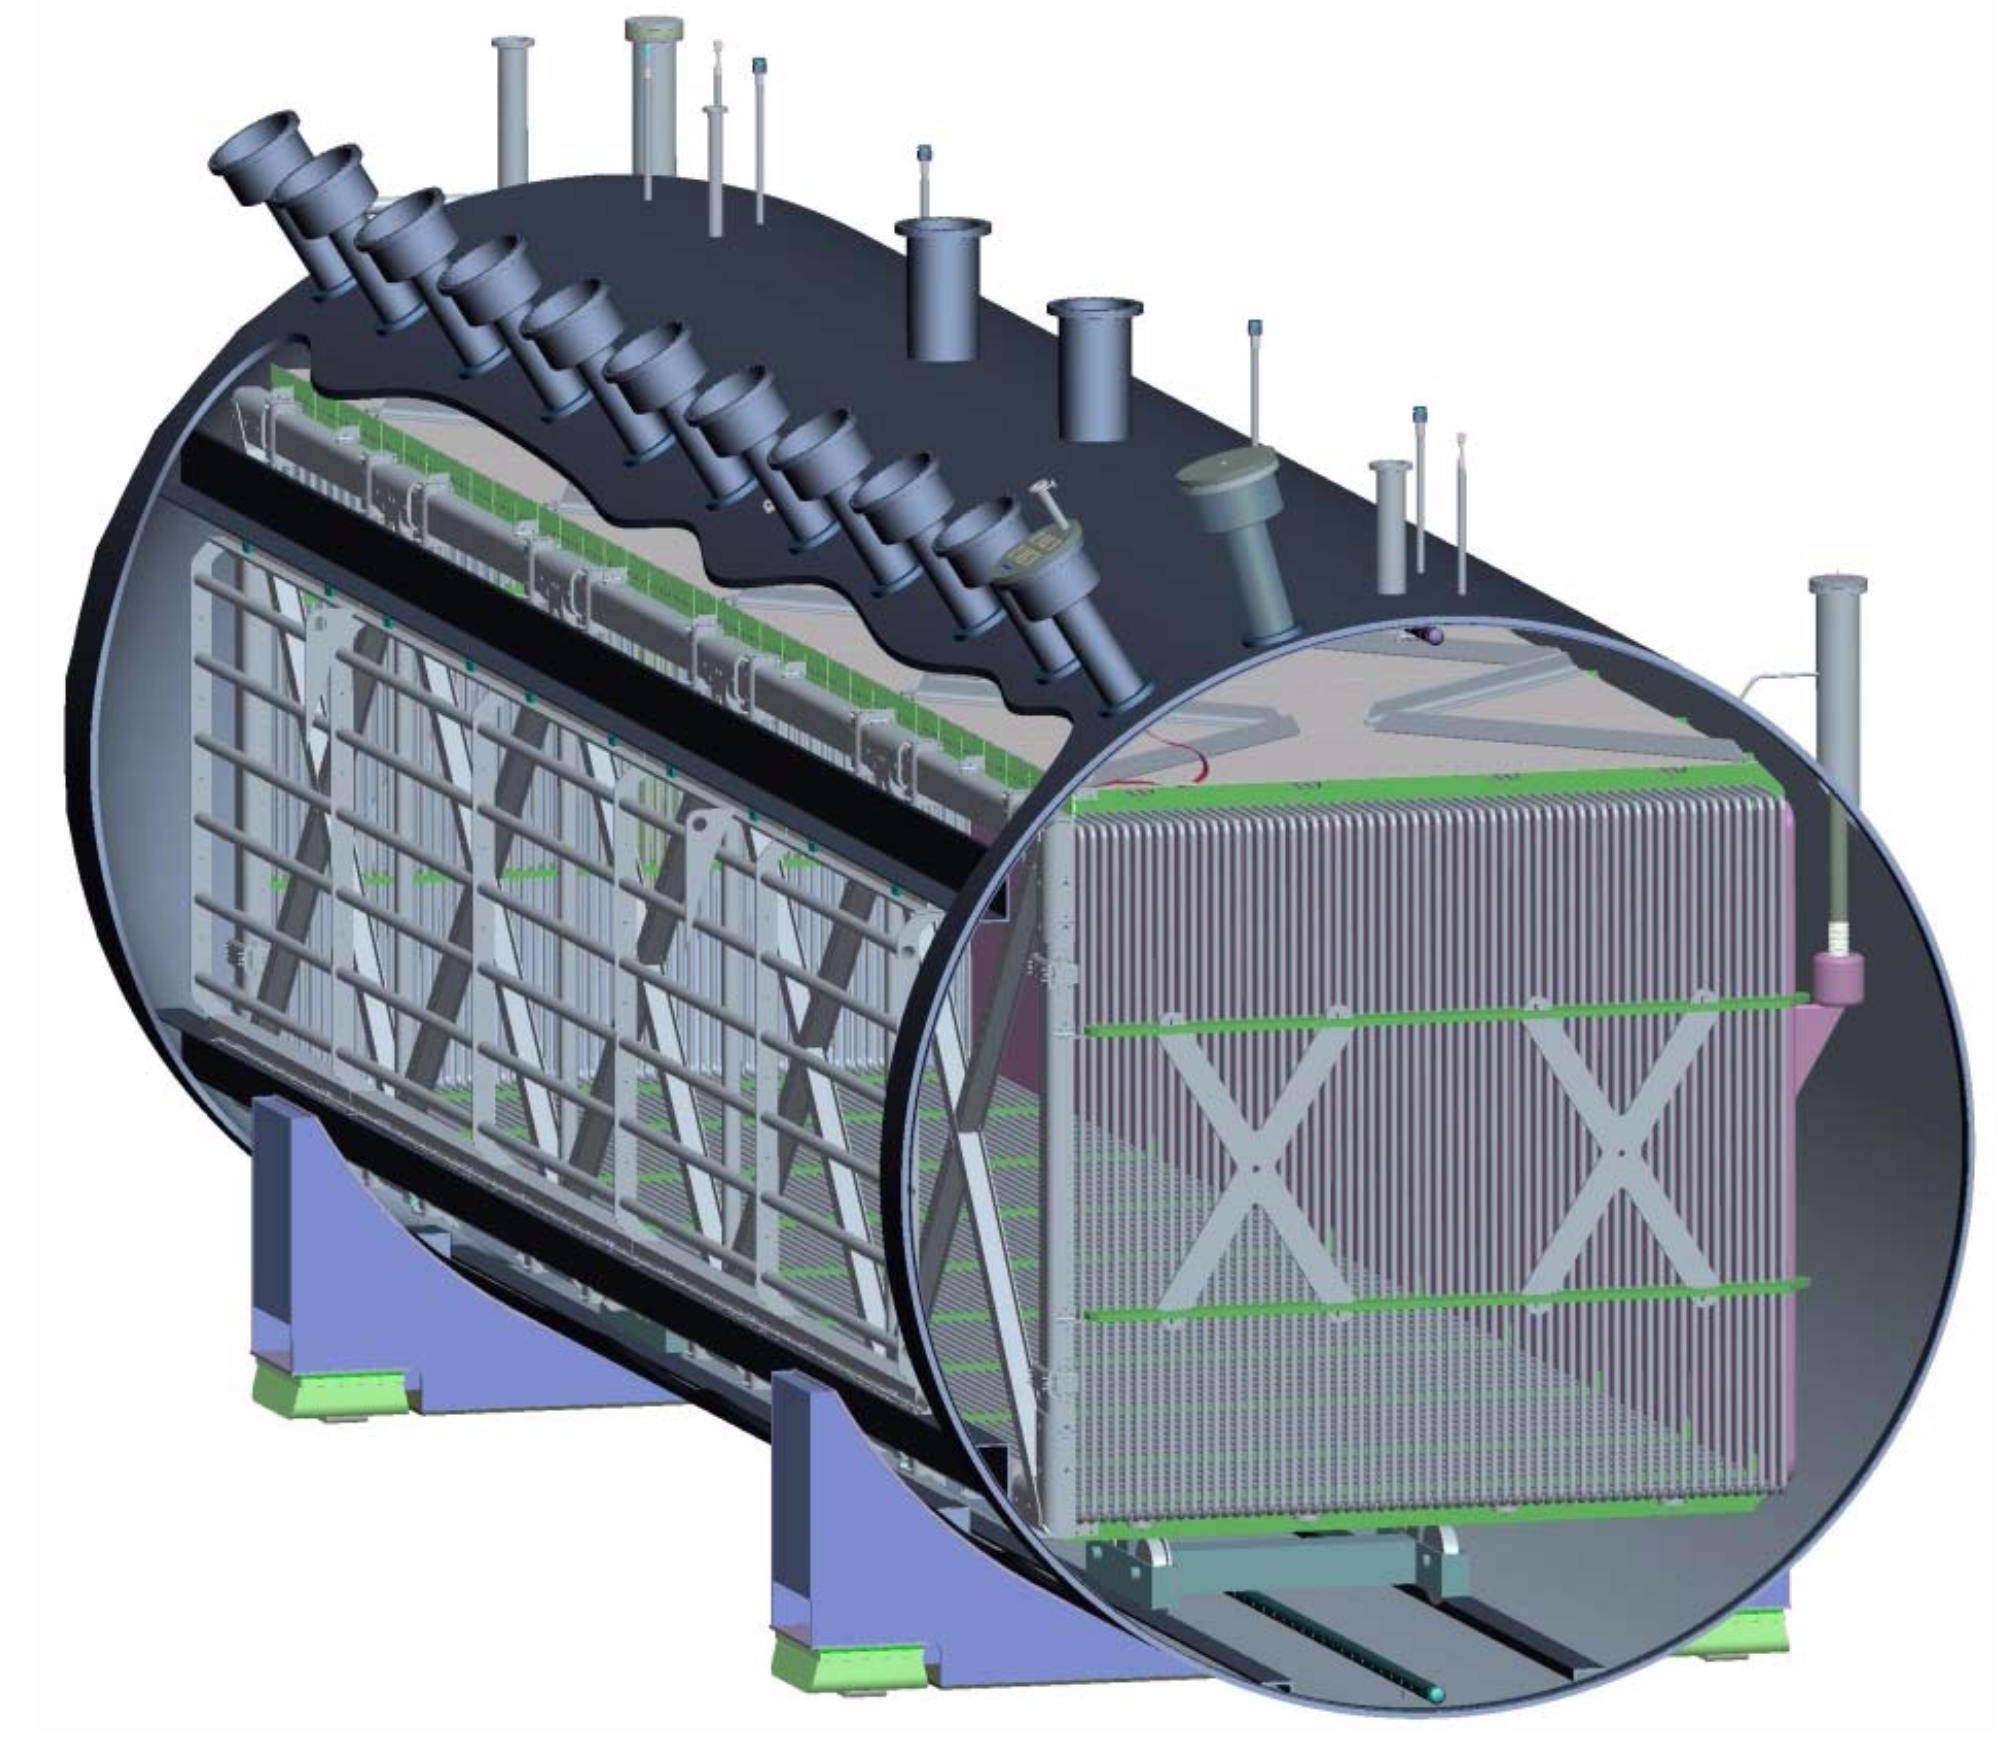
\includegraphics[width=0.7\textwidth]{Figures/cryo_3D_rendering.png} \\
\caption{\textit{A 3D rendering of the MicroBooNE detector. The rectangular time projection chamber (TPC) fits within the cylindrical cryostat. The feedthroughs along the top allow for the PMT and sense wire signals to be read out to the DAQ. Not shown are the photomultiplier tubes (PMTS) located on the wall behind the sense wire planes.}}\label{cryo_3D_rendering_fig}
\end{figure}


\begin{table}[!htb]
   \centering
     \caption{MicroBooNE LArTPC design parameters and nominal operating conditions.} 
    \begin{tabular}{lr} % Column formatting, @{} suppresses leading/trailing space
    \hline
    Parameter & Value \\
    \hline
    %\lartpc (active) dimensions ($h\times w\times l$) & 2.325 m $\times$ 2.560 m $\times$ 10.368 m\\
    %\lartpc (active) mass & 90 tons\\
   % \hline
    $\#$ Anode planes & 3\\
     Anode planes spacing& 3 mm \\
     Wire pitch & 3 mm  \\
     Wire type & SS, diam. 150 $\mu$m\\
     Wire coating & 2$\mu$m Cu, 0.1$\mu$m Ag\\
     Design Wire tension & 6.9N $\pm$ 1.0N\\
     $\#$ wires (total) & 8256 \\
     $\#$ Induction plane (U) wires & 2400 \\
     $\#$ Induction plane (V) wires & 2400 \\
     $\#$ Collection plane (Y) wires & 3456 \\
     Wire orientation (w.r.t. vertical) & +60$^{\circ}$,-60$^{\circ}$,0$^{\circ}$ (U,V,Y) \\
     \hline
     Cathode voltage (nominal) & -128 kV \\
     Bias voltages (U,V,Y) & -200 V, 0 V, +440 V \\
     Drift-field & 500 V/cm\\
   %  U-V gap field & 666.7 V/cm \\
    % V-Y gap field & 1466.7 V/cm \\
     Max. Drift Time, Cathode to U (at 500 V/cm) & 1.6 ms\\
    \hline
    $\#$ Field-cage steps & 64\\
    Ring-to-ring voltage step & 2.0 kV\\
    \hline
   \end{tabular}
   \label{UB_TPC_stats_table}
\end{table} 



\section{Light Collection System}
An important ingredient to the ultimate 3D reconstruction of particle interactions within a LArTPC is the light collection system. While the wire signals alone suffice to reconstruct 3D interactions, the absolute timing of the event (referred to as $t_0$) is unknown so there is ambiguity in the drift direction. Since the time scale with which scintillation light is created and propagates (nanoseconds) is orders of magnitude faster than that with which ionization electrons drift (milliseconds), measuring this light allows to clarify this ambiguity to high precision. Additionally, the scintillation light from interactions is relatively localized, and therefore combining the measured PMT signals with the physical position of the signal allows to match individual flashes of light with different interactions, which may have different $t_0$s. This is important to help tag and reject cosmic-induced backgrounds which may arrive outside of the expected beam neutrino arrival times.\\

The light collection system in MicroBooNE consists of 32 8-inch diameter Hamamatsu R5912-02mod cryogenic PMTs. These PMTs are mounted in a plane behind the three sense wire planes. The physical location of these PMTs is shown in Figure \ref{pmt_placement_fig}. These 32 PMTs provide 0.85\% photocathode coverage. Each PMT has mounted in front of it an acrylic plate, as shown in Figure \ref{pmt_mount_fig}. This plate is coated with TPB, an organic fluor which serves as a wavelength-shifting material. TPB absorbs the VUV scintillation light photons (128 nm wavelength in liquid argon) and re-emits it at visible wavelengths detectable by the PMTs, peaked at 425 nm.

\begin{figure}[ht!]
\centering
	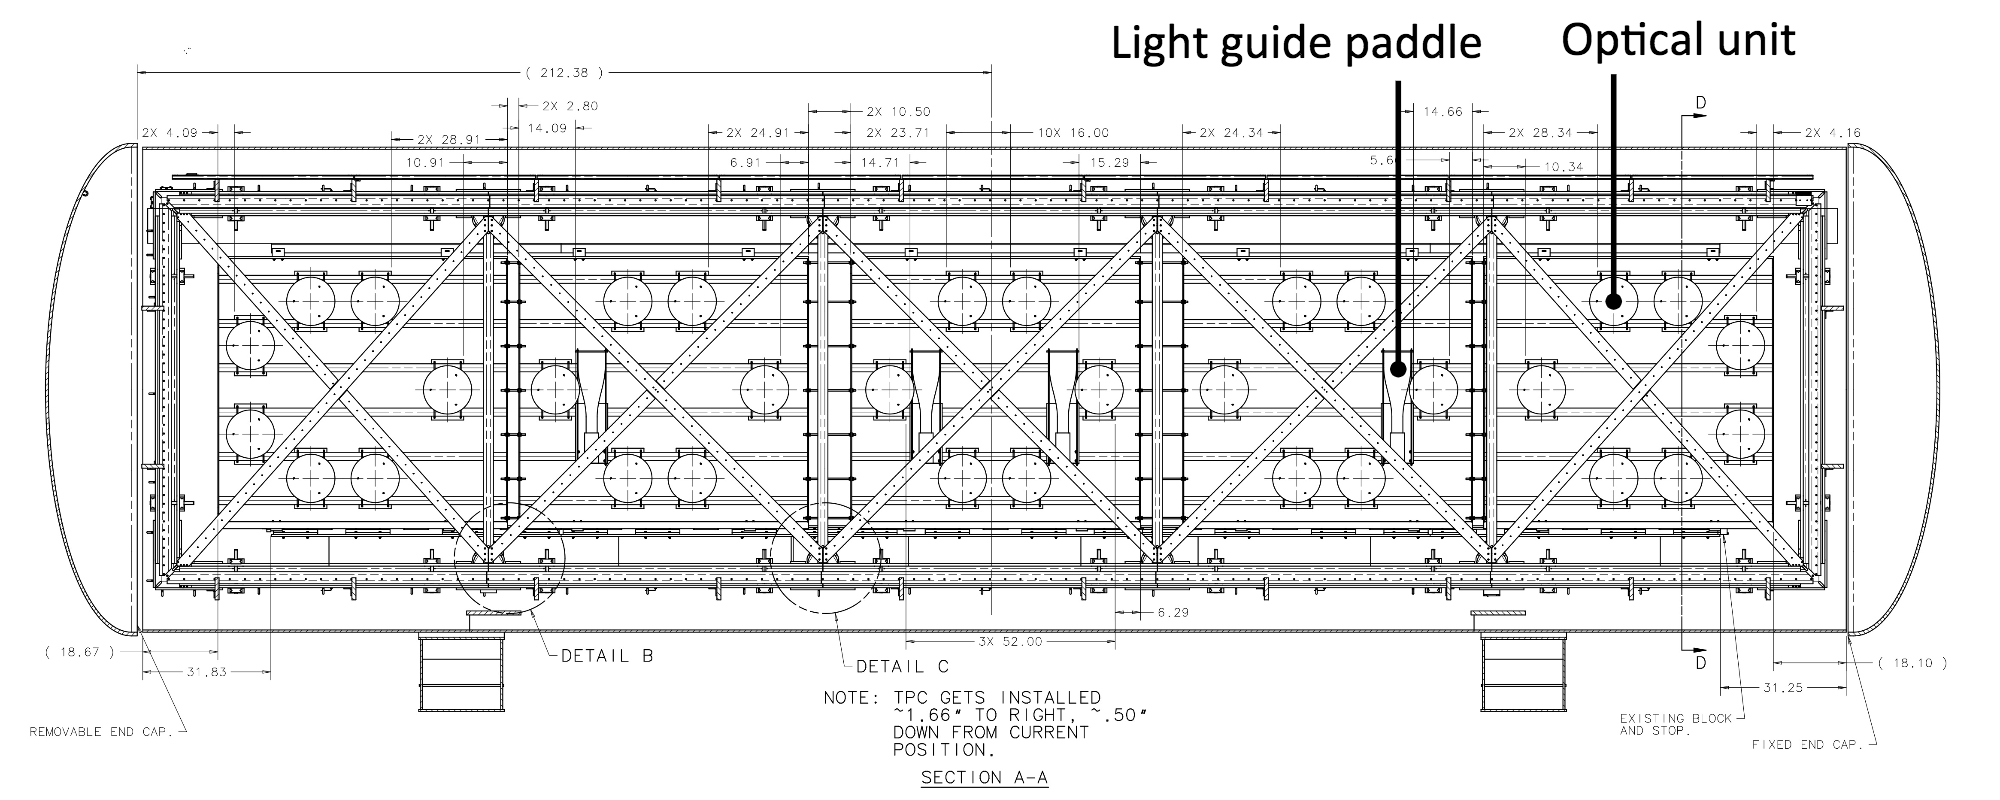
\includegraphics[width=0.9\textwidth]{Figures/pmt_placement.png} \\
\caption{\textit{A side-on view of the MicroBooNE detector showing the location of the 32 PMTs (labeled ``optical units'') and the four light guide paddles.}}\label{pmt_placement_fig}
\end{figure}


\begin{figure}[ht!]
\centering
	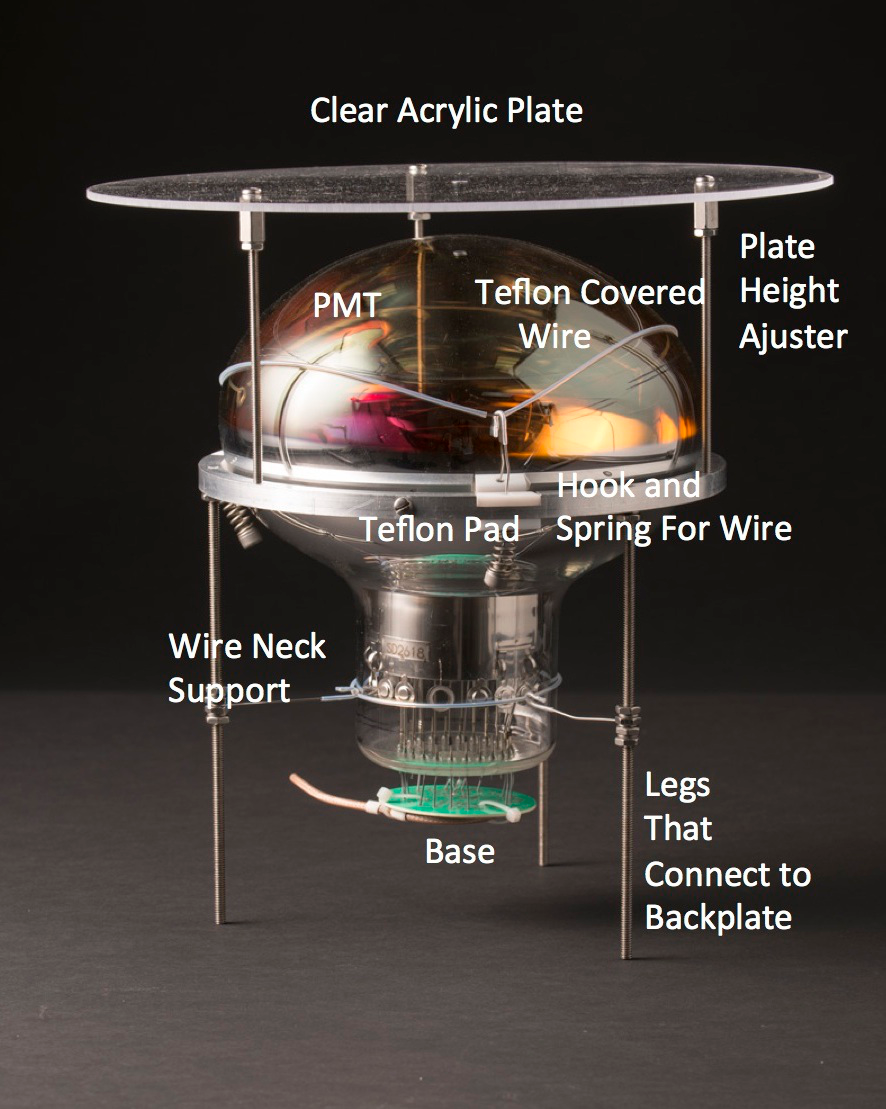
\includegraphics[width=0.6\textwidth]{Figures/mount_PMT_labeled.png} \\
\caption{\textit{A picture of one of the 8 inch Hamamatsu R5912-02mod cryogenic photomultiplier tubes (PMT) used in the MicroBooNE detector. Note the clear acrylic plate, which is coated with a wavelength-shifting organic fluor (TPB) before installation to convert the VUV liquid argon scintillation light into the visible spectrum, detectable by the PMT.}}\label{pmt_mount_fig}
\end{figure}


\section{Electronics, Readout, and Triggering}
Both of the two main subsystems of the MicroBooNE LArTPC (the TPC sense-wire planes and the optical PMTs) create analog signals which must be read out and digitized for use in analyses. This process involves amplification and shaping of the signals, and ultimately ends with the data acquisition (DAQ) software writing the digitized data to disk. While the readout is designed to have an additional data stream that continually writes to disk (designed with the hopes of measuring neutrino interactions from a potential future supernova explosion), the primary data stream reads out and stores signals only for a brief period of time when a hardware trigger is issued. The specifics of the readout and triggering for MicroBooNE are discussed in this section.\\

A schematic overview of the TPC and PMT signal processing and readout stages is shown in Figure \ref{readout_scheme_fig}. The analog signals from the 8256 sense wires in the TPC pass through CMOS analog front end ASICs which operate on cold motherboards at liquid argon temperatures. The signals are then shaped and amplified by cold intermediate amplifiers before passing through a warm feed-through. The signals are received by custom-designed LArTPC readout modules distributed over nine readout creates, which digitize the signals and process them. The TPC wire signals are digitized at 16 MHz and then down-sampled in the digitization process to 2 MHz. The TPC system reads out four 1.6 $ms$ frames of wire signal data associated with one event. This time is chosen based on how long it takes ionization electrons from the cathode side of the TPC to drift to the anode wires (roughly 1.6 $ms$ depending on drift field). Reading out one frame before a trigger is issued, along with two frames after ensures enough data is available to identify both a neutrino interaction, as well as all cosmic ray signals that arrive soon enough before or after the neutrino which need to be reconstructed in analyses.\\

\begin{figure}[ht!]
\centering
    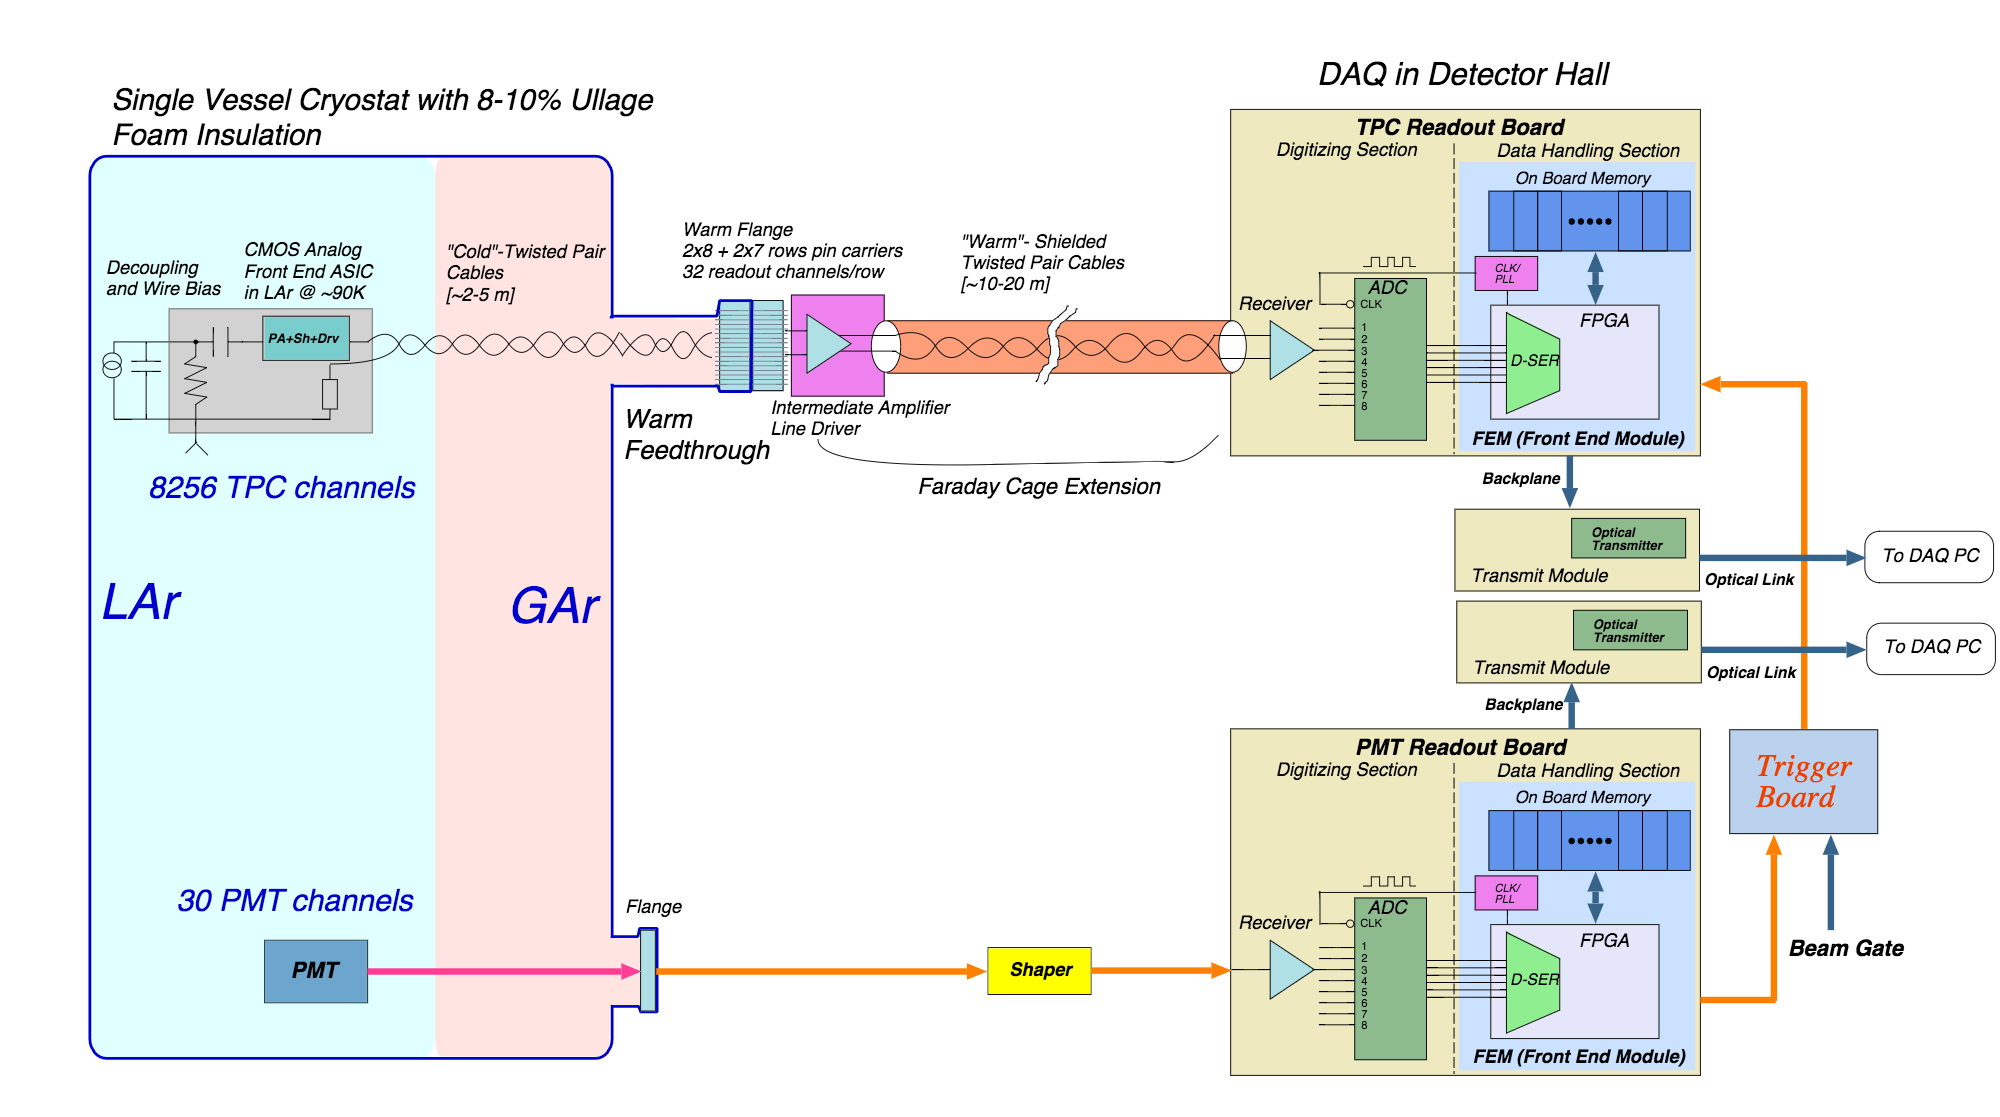
\includegraphics[width=0.95\textwidth]{Figures/UB_readout_scheme.png} \\
\caption{\textit{The MicroBooNE readout schematic. On the left are portions of the readout operating at argon temperatures. Signals pass through feedthroughs into warm electronics readout boards, unique for the TPC (sense wire signals) and the light collection system (PMT signals). These signals are combined with external timing signals from the accelerator to form triggers that initiate readout of all systems.}}\label{readout_scheme_fig}
\end{figure}

A similar process occurs for the PMT signals. The PMT signals undergo separate shaping with a 60 $ns$ peaking time to allow for digitization of several samples on the rising edge of a signal for more precise timing reconstruction abilities. The PMT signals are digitized at 64 MHz, but are not read out continuously during the same $4 \times 1.6$ $ms$ TPC readout time; only shaped PMT signals above a small discriminator threshold are read out and stored for later reconstruction. The PMT signals are split into high- and low- gain channels, to extend the dynamic range of the ADC.\\

The readout of both TPC and PMT systems are initiated by triggers formed in a separate trigger board located in a warm electronics readout crate. While many different triggers are used by MicroBooNE, the one relevant for this analysis is the BNB trigger. To form this trigger, a timing signal from the BNB accelerator is shaped and fed into the trigger board. The FPGA firmware in the PMT front end readout modules generates a PMT trigger when PMT signal multiplicity is greater than 1 and summed PMT pulse-height is more than 2 photo-electrons summed over all of the high gain PMT channels. If a PMT trigger is issued by the firmware in coincidence with the $1.6 \mu s$ beam gate window from the accelerator, a BNB trigger is generated by the trigger board. This trigger signal is fanned-out to all readout crates (TPC and PMT), instructing them to initiate a readout simultaneously. Once the readout is complete, the data from each readout crate is packaged and shipped to the DAQ software, which assembles all of the data into one event in memory, which is saved to disk and eventually used in reconstruction and analysis. Note that ultimately, the MicroBooNE collaboration has moved towards using a software- based trigger for its beam-based analyses.

%\cite{UBDetectorPaper}